%%%%%%%%%%%%%%%%%%%%%%%%%%%%%%%%%%%%%%%%%%%%%%%%%%%%%%%%%%%%%%%%
%%		                                                      %%
%% aGreekPrimer, Italian translation 2016.12 - 2017          %%
%%		                                                      %%
%% From:  Clarence W. Gleason, A Greek Primer                 %%
%%        (1903, New York, American Book Company)             %%
%%		                                                      %%
%%		  https://archive.org/details/greekprimer00glea       %%
%%		                                                      %%
%% Translated by g.p.ciceri <gp.ciceri@gmail.com>             %%
%% ---------------------------------------------------------- %%
%% This translation is Licensed under                         %%
%% Creative Commons Attribution-ShareAlike 4.0 International  %%
%% https://creativecommons.org/licenses/by-sa/4.0/            %%
%%		                                                      %%
%%%%%%%%%%%%%%%%%%%%%%%%%%%%%%%%%%%%%%%%%%%%%%%%%%%%%%%%%%%%%%%%

% ᾶῖῶῆῦ  
% ἀἰὐἐὀὠἠ 
% ὰὲὶὸὺὼὴ 
% ἁἱὑὁὡἡῥ
% άέίόύήώΆΉ
% ἂἒὒἲὂὢἢὒἚἊ
% ἃἳὓὃἣὣἓἋἛ
% ἄἔἴὄὔὤἤἌἬ
% ἅἕἵὅὕὥἥἍἭ
% ἆὦἶἦὖἯἏὯἇὧἷἧὗἯἏὯ 

% ᾳῃῳ
% ᾱῑῡ
% ᾀᾐᾠ
% ᾰῐῠ
% ᾂᾒᾢ
% ϊ ϋ
% ᾄᾔᾤ
% ΰ ΐ
% ᾆᾖᾦ
% ᾲῂῲ
% ᾴῄῴ
% ᾷῇῷ
% ᾳῃῳ
% ᾱῑῡ
% ᾰῐῠ

% āēīōū
% ăĕĭŏŭ


\documentclass[nols]{tufte-handout}

%\geometry{showframe} % display margins for debugging page layout

\usepackage{fontspec}
\usepackage{ifxetex}
\setmainfont[Path=./fonts/palatino-linotype/, ItalicFont=palai.ttf, BoldFont=palab.ttf]{pala.ttf}


% \defaultfontfeatures{Mapping=tex-text}
% \setromanfont[Path=./fonts/TeX-Gyre-Schola/,Mapping=tex-text]{TeX Gyre Schola}
% \setsansfont[Path=./fonts/TeX-Gyre-Heros/,Scale=MatchLowercase,Mapping=tex-text]{TeX Gyre Heros}
% \setmonofont[Path=./fonts/TeX-Gyre-Cursor/,Scale=MatchLowercase]{TeX Gyre Cursor}

\usepackage{lipsum}
\usepackage{url}
\usepackage{longtable}
\usepackage{stackengine}

\usepackage{graphicx} % allow embedded images
  \setkeys{Gin}{width=\linewidth,totalheight=\textheight,keepaspectratio}
  \graphicspath{{graphics/}} % set of paths to search for images
\usepackage{amsmath}  % extended mathematics
\usepackage{booktabs} % book-quality tables
\usepackage{units}    % non-stacked fractions and better unit spacing
\usepackage{multicol} % multiple column layout facilities
\usepackage{lipsum}   % filler text
\usepackage{fancyvrb} % extended verbatim environments
  \fvset{fontsize=\normalsize}% default font size for fancy-verbatim environments

% Standardize command font styles and environments
\newcommand{\doccmd}[1]{\texttt{\textbackslash#1}}% command name -- adds backslash automatically
\newcommand{\docopt}[1]{\ensuremath{\langle}\textrm{\textit{#1}}\ensuremath{\rangle}}% optional command argument
\newcommand{\docarg}[1]{\textrm{\textit{#1}}}% (required) command argument
\newcommand{\docenv}[1]{\textsf{#1}}% environment name
\newcommand{\docpkg}[1]{\texttt{#1}}% package name
\newcommand{\doccls}[1]{\texttt{#1}}% document class name
\newcommand{\docclsopt}[1]{\texttt{#1}}% document class option name
\newenvironment{docspec}{\begin{quote}\noindent}{\end{quote}}% command specification environment

% concetti morfosintattici
\usepackage{xspace} 
\newcommand{\noun}{\textsc{sostantivo}\xspace}
\newcommand{\nouns}{\textsc{sostantivi}\xspace}
\newcommand{\adject}{\textsc{aggettivo}\xspace}
\newcommand{\adjects}{\textsc{aggettivi}\xspace}
\newcommand{\gnumber}{\textsc{numero}\xspace}
\newcommand{\gnumbers}{\textsc{numeri}\xspace}
\newcommand{\gender}{\textsc{genere}\xspace}
\newcommand{\genders}{\textsc{generi}\xspace}
\newcommand{\gcase}{\textsc{caso}\xspace}
\newcommand{\gcases}{\textsc{casi}\xspace}
\newcommand{\tense}{\textsc{tempo}\xspace}
\newcommand{\mood}{\textsc{modo}\xspace}
\newcommand{\gverb}{\textsc{verbo}\xspace}
\newcommand{\gverbs}{\textsc{verbi}\xspace}
\newcommand{\adjective}{\textsc{aggettivo}\xspace}
\newcommand{\nom}{\textsc{nom}\xspace}
\newcommand{\gen}{\textsc{gen}\xspace}
\newcommand{\dat}{\textsc{dat}\xspace}
\newcommand{\acc}{\textsc{acc}\xspace}
\newcommand{\voc}{\textsc{voc}\xspace}
\newcommand{\gexit}{\textsc{uscita}\xspace}
\newcommand{\gexits}{\textsc{uscite}\xspace}
\newcommand{\declinazione}{\textsc{declinazione}\xspace}
\newcommand{\masc}{\textsc{maschile}\xspace}
\newcommand{\femm}{\textsc{femminile}\xspace}
\newcommand{\neut}{\textsc{neutro}\xspace}

\newcommand{\indic}{\textsc{indicativo}\xspace}
\newcommand{\imper}{\textsc{imperativo}\xspace}
\newcommand{\gcong}{\textsc{congiuntivo}\xspace}
\newcommand{\ott}{\textsc{ottativo}\xspace}
\newcommand{\partic}{\textsc{participio}\xspace}
\newcommand{\infin}{\textsc{infinito}\xspace}

\newcommand{\pres}{\textsc{presente}\xspace}
\newcommand{\imperf}{\textsc{imperfetto}\xspace}
\newcommand{\aor}{\textsc{aoristo}\xspace}
\newcommand{\fut}{\textsc{futuro}\xspace}

\newcommand{\sing}{\textsc{singolare}\xspace}
\newcommand{\plur}{\textsc{plurale}\xspace}
\newcommand{\dual}{\textsc{duale}\xspace}


% italianitudini
\renewcommand{\figurename}{Figura}
\renewcommand{\tablename}{Tabella}
\renewcommand{\contentsname}{Indice}

% fix per un qualche problema
\ifxetex
  \newcommand{\textls}[2][5]{%
    \begingroup\addfontfeatures{LetterSpace=#1}#2\endgroup
  }
  \renewcommand{\allcapsspacing}[1]{\textls[15]{#1}}
  \renewcommand{\smallcapsspacing}[1]{\textls[10]{#1}}
  \renewcommand{\allcaps}[1]{\textls[15]{\MakeTextUppercase{#1}}}
  \renewcommand{\smallcaps}[1]{\smallcapsspacing{\scshape\MakeTextLowercase{#1}}}
  \renewcommand{\textsc}[1]{\smallcapsspacing{\textsmallcaps{#1}}}
\fi

\title{A Greek Primer. Introduzione al Greco Antico \newline Lezione VIΙI - Declinazione in A. Nomi in ᾰ (alfa breve).}

\author[gpciceri]{a cura di Milagathòs: Milo's help to enjoy humanities\marginnote{\url{http://www.milagathos.com}}
}

\date{4 Gennajo 2017} % without \date command, current date is supplied


\begin{document}

\maketitle% this prints the handout title, author, and date

\begin{marginfigure}[-3.0cm]
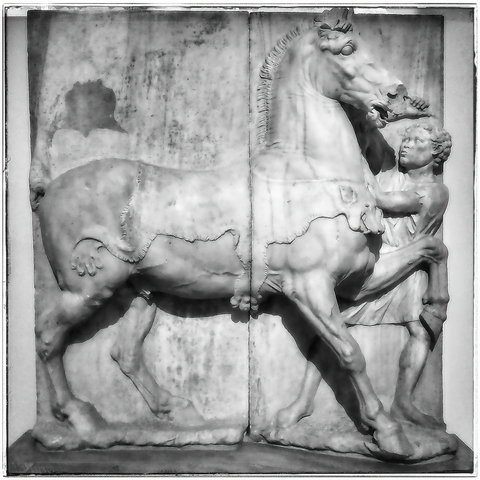
\includegraphics{smallthumb-lesson_I.jpeg}
\setfloatalignment{b}
\end{marginfigure}


\begin{abstract}
\noindent
Queste lezioni si articolano in \textsc{elementi grammaticali}, 
espressi sommariamente, seguiti da \textsc{vocabolari} per il lessico di base 
e da \textsc{frasi da tradurre} dal greco e in greco. 
\
L'approccio è quello del testo-laboratorio di morfosintassi: 
si presenta punto per punto - riprendendone la numerazione - 
l'esposizione di Gleason\cite{gleason1903}.\\
\bigskip
\noindent
Lezione VIII: la declinazione in A), nomi femminili in ᾰ, vocabolario, esercizi.
\end{abstract}

%\printclassoptions

\newthought{97.} Alcuni nomi femminili di questa declinazione terminano in \textbf{ᾰ}, 
che viene allungata in \textbf{η} al genitivo e al dativo singolare\sidenote{in particolare dopo  \textbf{σ, λλ, ττ} o una doppia consonante.}, 
a meno che la \textbf{ᾰ} non sia preceduta da \textbf{ε, ι} o \textbf{ρ}.

\newthought{98. Modelli}

\begin{fullwidth}
\begin{table}[!htbp]
  \centering
  \begin{tabular}{l l l l l l}
    %\toprule
	\multicolumn{6}{c}{\textsc{parole guida}} \\
	& \textbf{Μοῦσα,} & \multicolumn{3}{c}{\textbf{ἡ μακρὰ γέφῡρα,}} & \textbf{ἅμαξα,} \\
	& \textit{Musa,} \textsc{F.} & \multicolumn{3}{c}{\textit{il lungo ponte}} & \textit{Carro,} \textsc{F.}\\
   
	\multicolumn{6}{c}{\textsc{singolare}} \\
    \textsc{n.} & \textbf{Μοῦσα}  & \textbf{ἡ}   & \textbf{μακρὰ}  & \textbf{γέφῡρα}  & \textbf{ἅμαξα} \\
    \textsc{g.} & \textbf{Μούσης} & \textbf{τῆς} & \textbf{μακρᾶς} & \textbf{γέφύρᾱς} & \textbf{ἁμάξης} \\
    \textsc{d.} & \textbf{Μούσῃ}  & \textbf{τῇ}  & \textbf{μακρᾷ}  & \textbf{γέφύρᾳ}  & \textbf{ἁμάξῃ} \\
	\textsc{a.} & \textbf{Μοῦσαν} & \textbf{τὴν} & \textbf{μακρὰν} & \textbf{γέφῡραν} & \textbf{ἅμαξαν} \\
	\textsc{v.} & \textbf{Μοῦσα}  & \textemdash  & \textbf{μακρὰ}  & \textbf{γέφῡρα}  & \textbf{ἅμαξα} \\
	
	\multicolumn{6}{c}{\textsc{plurale}} \\
	\textsc{n.v.} & \textbf{Μοῦσαι} & \textbf{αἱ}   & \textbf{μακραὶ}  & \textbf{γέφῡραι}   & \textbf{ἅμαξαι}\\
    \textsc{g.} & \textbf{Μουσῶν}  & \textbf{τῶν}  & \textbf{μακρῶν}  & \textbf{γέφῡρῶν}  & \textbf{ἁμαξῶν} \\
    \textsc{d.} & \textbf{Μούσαις} & \textbf{ταῖς} & \textbf{μακραῖς} & \textbf{γεφύραις} & \textbf{ἁμάξαις}  \\
	\textsc{a.} & \textbf{Μούσᾱς} & \textbf{τὰς}  & \textbf{μακρὰς}  & \textbf{γεφύρᾱς}  & \textbf{ἁμάξᾱς} \\
    %\bottomrule
  \end{tabular}
  \label{tab:normaltab}
  %\zsavepos{pos:normaltab}
\end{table}
\end{fullwidth}

\newthought{Esercizio}
\begin{itemize}
\item[\textsc{1.}] In \textbf{Μοῦσα, γέφῡρα, ἅμαξα,} osserva e spiega i cambiamenti degli accenti. 
\end{itemize}

\newpage

\newthought{99. Vocabolario}

\begin{multicols}{2}
    \noindent \hangindent=1em \textbf{ἅμαξα, ἡ} \textit{carro}.  \\
    \noindent \hangindent=1em \textbf{βασίλεια, ἡ} \textit{regina}.  \\
    \noindent \hangindent=1em \textbf{γέφῡρα, ἡ} \textit{ponte}.  \\
    \noindent \hangindent=1em \textbf{θηρίον, τό} \textit{animale selvaggio}.  \\
    \noindent \hangindent=1em \textbf{θύρᾱ, ἡ} \textit{porta}.  \\
    \noindent \hangindent=1em \textbf{λόγχη, ἡ} \textit{lancia}.  \\
    \noindent \hangindent=1em \textbf{μάχαιρα, ἡ} \textit{spada}.  \\
    \noindent \hangindent=1em \textbf{Μοῦσα, ἡ} \textit{Musa}.  \\
	
    \noindent \hangindent=1em \textbf{ὁδός, ἡ} \textit{via, strada, marcia}.  \\
    \noindent \hangindent=1em \textbf{πηγή, ἡ} \textit{primavera,} pl. \textit{fonte}.  \\
	
	\noindent \hangindent=1em \textbf{διώκω,} fut. \textbf{διώξω,} 
	aor. \textbf{ἐδιώξα,} \textit{inseguire}. \\ 
	\noindent \hangindent=1em \textbf{θηρεύω,} fut. \textbf{θηρεύσω,} 
	aor. \textbf{ἐθήρευσα,} \textit{cacciare}. \\ 
	
    \noindent \hangindent=1em \textbf{ταχέως,} avv.,\textit{velocemente}.  \\
	\noindent \hangindent=1em \textbf{διά,} prep. con \gen \textit{attraverso}; con \acc \textit{a quale scopo}.  \\
	
\end{multicols}

\newthought{Osservazione}
\begin{itemize}
\item[\textsc{1.}] Per indicare il genere del nome, si usa normalmente scriverlo con l'articolo.
In questo modo \textbf{ὁδός, ἡ} mostra che \textbf{ὁδός} è femminile. 
\end{itemize}

\newthought{100. Traduci:}
\textsc{1.}~ἐπὶ τῆς ἁμάξες. \quad
\textsc{2.}~ἐκ τῆς πηγῆς. \quad
\textsc{3.}~ἡ τῆς χώρᾱς βασίλεια. \quad
\textsc{4.}~λόγχαις μακραῖς. \quad
\textsc{5.}~τῶν σοφῶν Μουσῶν. \quad

\newthought{101.}
\textsc{1.}~αἱ τῶν οἰκιῶν θύραι ἦσαν μικραί. \quad
\textsc{2.}~ἐν δὲ τῷ χωρίῳ ἔμενον πέντε ἄνθρωποι ἀγαθοί. \quad
\textsc{3.}~τὰ δὲ θηρία ἔφευγε ταχέως διὰ τοῦ ποταμοῦ. \quad
\textsc{4.}~τίς ἄξει τοὺς λίθους ἐπὶ μακρῶν ἁμαξῶν; \quad
\textsc{5.}~ἡ δὲ βασίλεια ἔπεμψεν ἀγγέλους ἐπὶ τὴν ἄκραν. \quad
\textsc{6.}~οἱ δὲ ἐθήρευον ἐν τῷ πεδίῳ. \quad
\textsc{7.}~τὰ γὰρ παιδία ἐδίωξε τοὺς ἵππους εἰς τὴν οἰκίαν. \quad
\textsc{8.}~οἱ δὲ υἱοὶ τῆς βασιλείας εἶχον λόγχας καὶ μαχαίρας. \quad
\textsc{9.}~ἡ ὁδὸς ἄγει ἐπὶ τὰς τοῦ ποταμοῦ πηγάς.

\newthought{102. Scrivi in Greco:}
\textsc{1.}~Chi ha distrutto i ponti? \quad
\textsc{2.}~Essi sacrificavano alle Muse. \quad
\textsc{3.}~Erano sagge le parole dei fanciulli? \quad
\textsc{4.}~Egli lasciò, tu colpisti, io manderò, noi inseguiremo. \quad

\begin{figure*}[!b]
  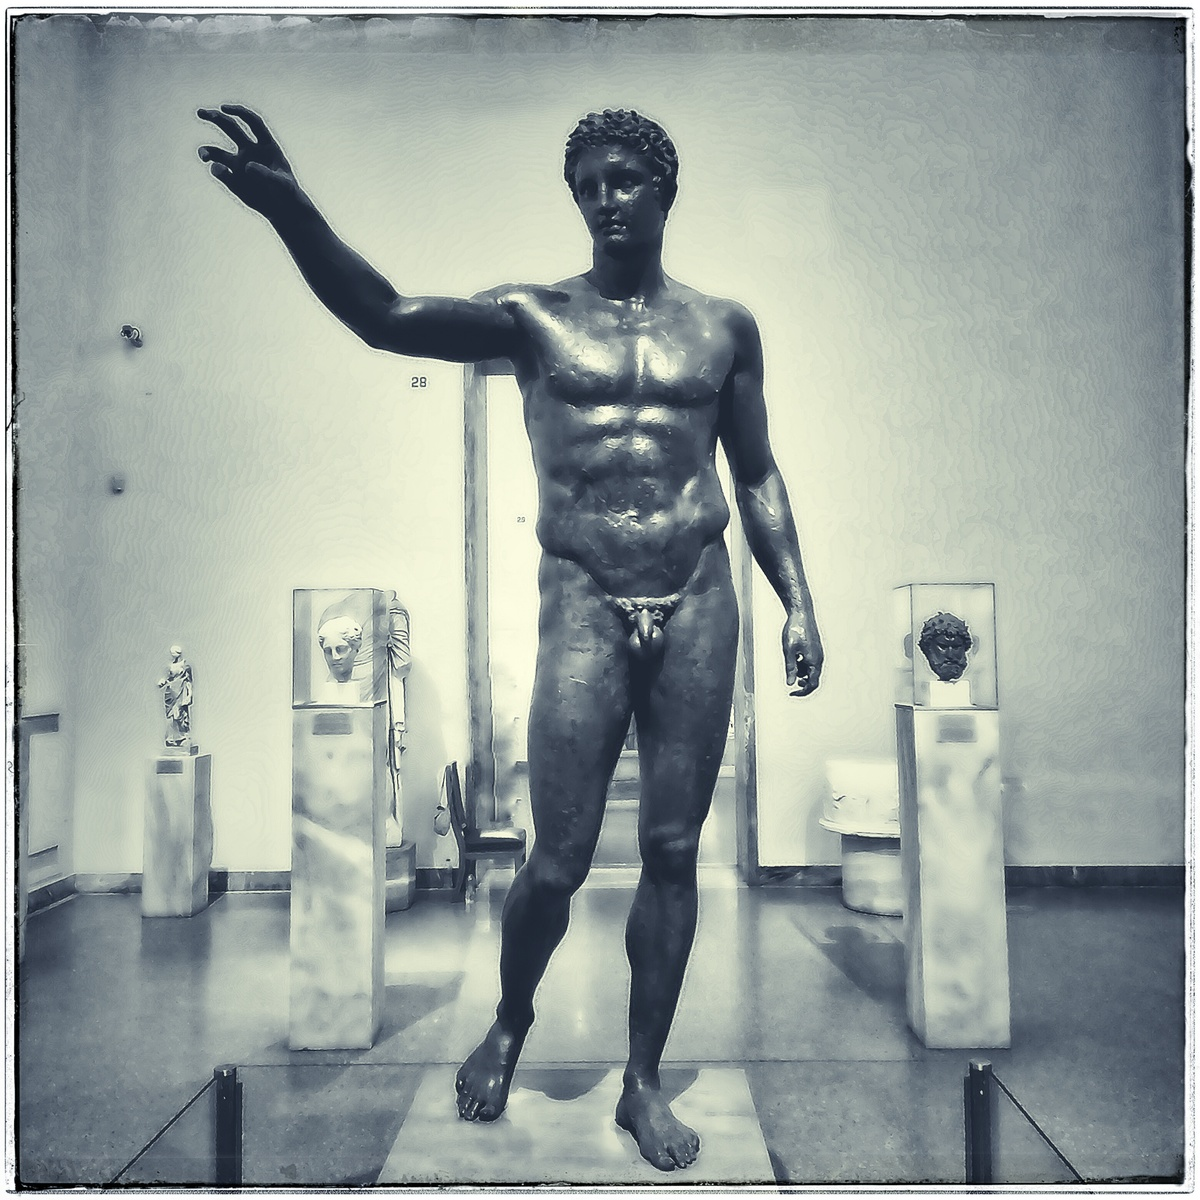
\includegraphics{thumb-lesson_VIII.jpeg}
  \caption{Museo Nazionale di Archeologia di Atene}
  \label{fig:textfig}
  %\zsavepos{pos:textfig}
  %\setfloatalignment{b}
\end{figure*}

 

\nobibliography{greekBiblio}
\bibliographystyle{alpha}


\end{document}
